\chapter{Results}

\section{Proximal Policy Optimization (PPO)}

PPO is an on policy, stochastic and policy gradient based reinforcement learning method \cite{ppo}. The objective function of PPO is 

\begin{equation}
L^{CLIP} (\theta) = \hat{E}_t \left[ min(r_t(\theta) \hat{A}_t, clip(r_t(\theta), 1 - \epsilon, 1 + \epsilon) \hat{A}_t) \right]
\end{equation}

Where
\begin{itemize}
	\item $\theta$ is the policy parameter
	\item $\hat{E}_t$ denotes the empirical expectation over timesteps
	\item $r_t$ is the ratio of probability under the new and old policies, respectively
	\item $\hat{A}_t$ is the estimated advantage at time $t$
	\item $\epsilon$ is a hyperparameter, usually 0.1 or 0.2
\end{itemize}

\subsection{Architecture}
PPO requires two neural networks, value network to calculate advantage of taking an action and policy network for predicting mean and variance of an action to maximize reward at a given state. We use 3 layer CNN for extracting features from image of gripper camera. The input image shape is $84 \times 84 \times 4$. Fourth channel is depth value. The value network and policy network can share this 3 layer CNN for feature extraction. But since loss functions of value network and policy network are different, sharing the CNN layers might optimize the CNN layers for either value or policy network. This can be fixed by scaling the loss functions of value and policy network to same scale.

\begin{figure}[H]
	\centering
	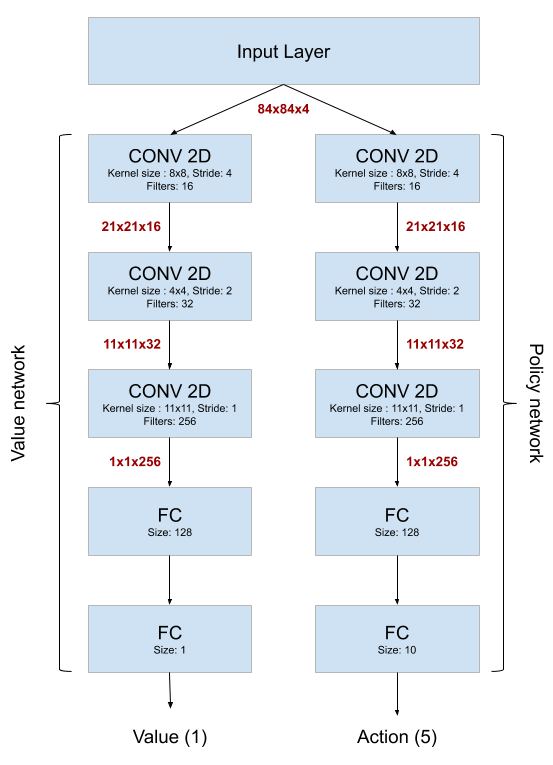
\includegraphics[scale=0.5]{ppo-arch}
	\caption{PPO network architecture}
\end{figure}

\subsection{Table clearing environment}
\subsubsection{Simulation}
After training PPO agent on table clearing environment using 8 core 42GB RAM Nvidia T4 GPU system for 4M timesteps, results are shown below

\begin{figure}[H]
	\centering
	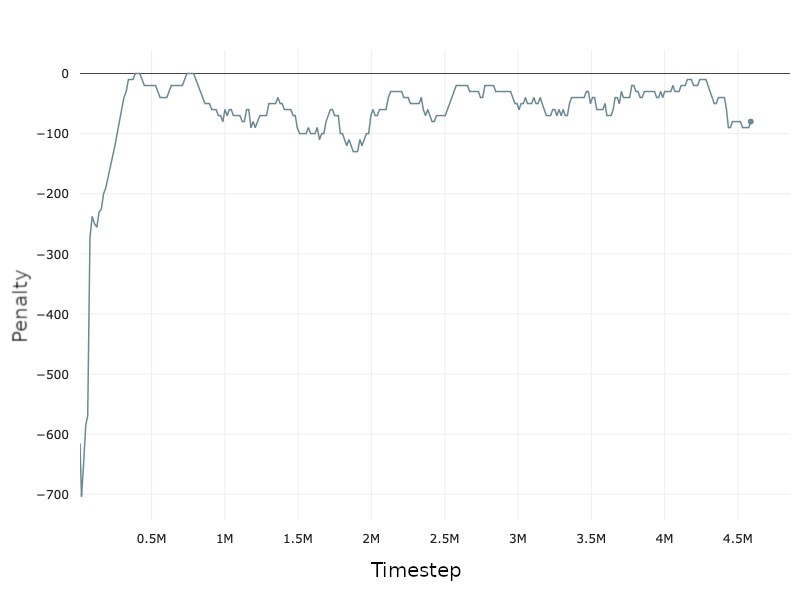
\includegraphics[scale=0.4]{ppo-simulation-collision-penalty}
	\caption{Collision penalty. Optimum value is 0}
\end{figure}

\begin{figure}[H]
	\centering
	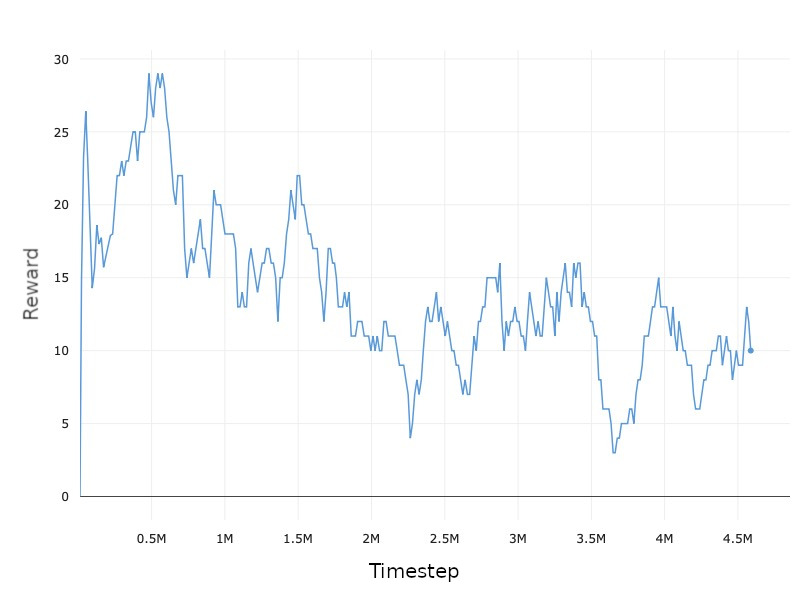
\includegraphics[scale=0.4]{ppo-simulation-grasp-reward}
	\caption{Grasp reward. Optimum value is 100}
\end{figure}

\begin{figure}[H]
	\centering
	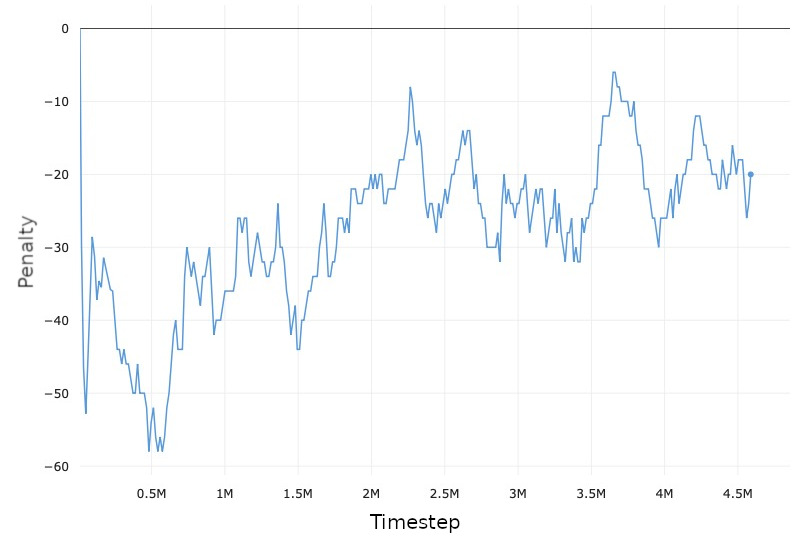
\includegraphics[scale=0.4]{ppo-simulation-drop-penalty}
	\caption{Drop penalty. Optimum value is 100}
\end{figure}

\begin{figure}[H]
	\centering
	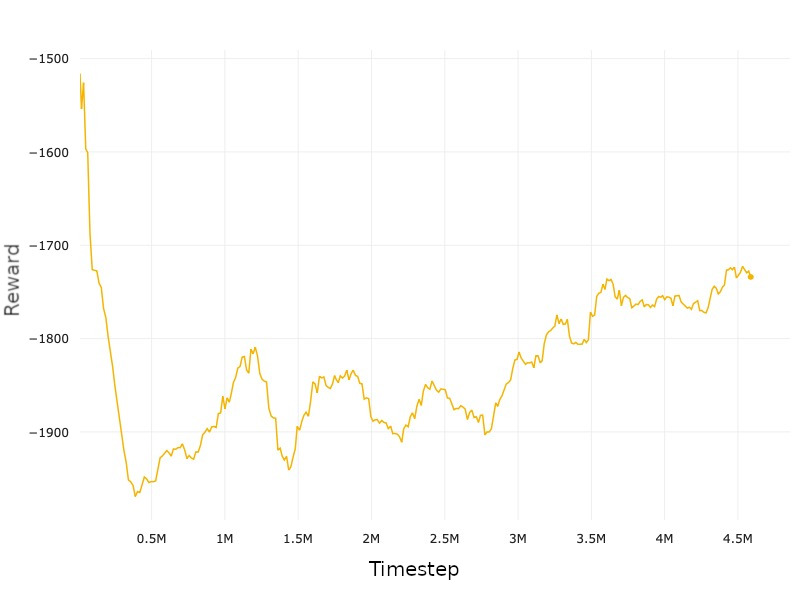
\includegraphics[scale=0.4]{ppo-simulation-reward-mean}
	\caption{Mean episode reward. Optimum value $\ge 200$}
\end{figure}

For attaining optimum reward, network needs to be trained for approximately 80M timesteps.